\documentclass[tikz,border=10pt]{standalone}
\usepackage{mathpazo}
\usepackage{tikz}
\usetikzlibrary{shapes,arrows,positioning,calc,fit,backgrounds}

\begin{document}

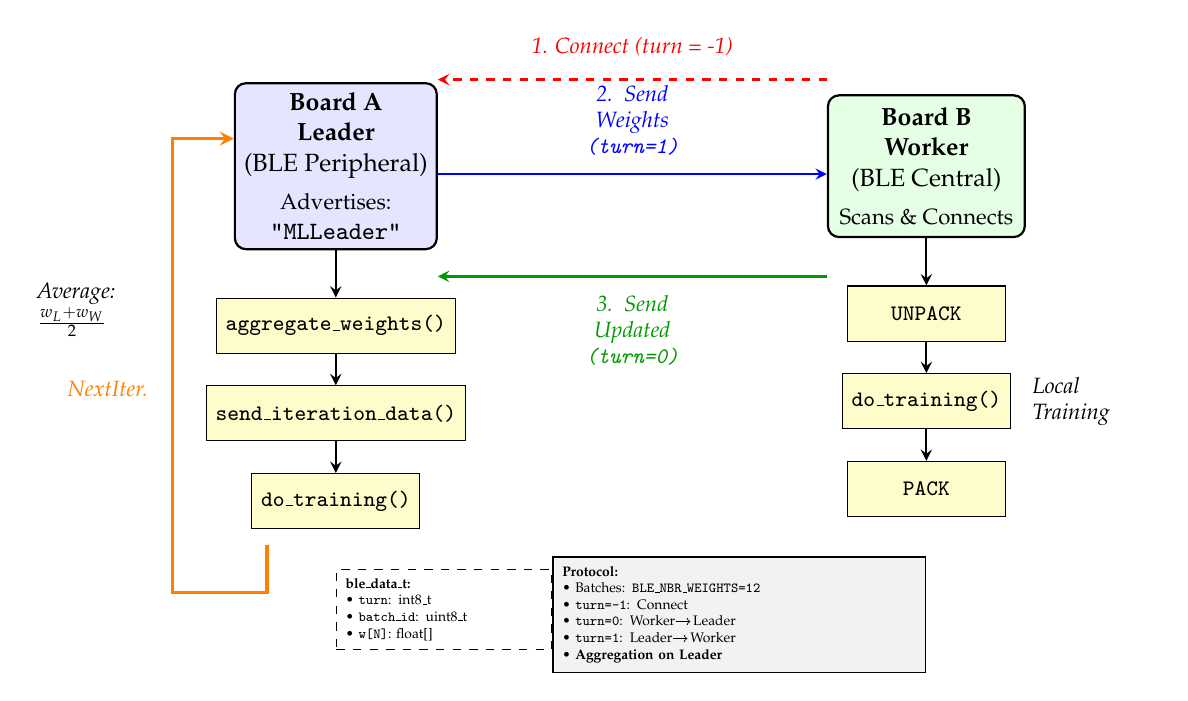
\begin{tikzpicture}[
    node distance=1.0cm,
    box/.style={rectangle, draw, thick, minimum width=2.5cm, minimum height=1.8cm, align=center, rounded corners, font=\small},
    leader/.style={box, fill=blue!10},
    worker/.style={box, fill=green!10},
    process/.style={rectangle, draw, fill=yellow!20, minimum width=2.0cm, minimum height=0.7cm, align=center, font=\footnotesize},
    arrow/.style={->, >=stealth, thick},
    dashedarrow/.style={->, >=stealth, thick, dashed},
    label/.style={font=\footnotesize\itshape}
]

% Board A (Leader)
\node[leader] (boardA) at (0,0) {
    \textbf{Board A}\\
    \textbf{Leader}\\
    (BLE Peripheral)\\[0.1cm]
    \footnotesize Advertises:\\
    \texttt{"MLLeader"}
};

% Board B (Worker)
\node[worker] (boardB) at (7.5,0) {
    \textbf{Board B}\\
    \textbf{Worker}\\
    (BLE Central)\\[0.1cm]
    \footnotesize Scans \& Connects
};

% Process boxes for Board A (Leader)
\node[process, below=0.6cm of boardA] (aggA) {\texttt{aggregate\_weights()}};
\node[process, below=0.4cm of aggA] (sendA) {\texttt{send\_iteration\_data()}};
\node[process, below=0.4cm of sendA] (trainA) {\texttt{do\_training()}};

% Process boxes for Board B (Worker)
\node[process, below=0.6cm of boardB] (unpackB) {\texttt{UNPACK}};
\node[process, below=0.4cm of unpackB] (trainB) {\texttt{do\_training()}};
\node[process, below=0.4cm of trainB] (packB) {\texttt{PACK}};

% Arrows showing communication flow
% Step 1: Initial connection (topmost)
\draw[dashedarrow, red] ($(boardB.west)+(0,1.1)$) -- node[above, label, yshift=5pt] {1. Connect (turn = -1)} ($(boardA.east)+(0,1.1)$);

% Step 2: Leader sends aggregated weights to Worker (middle top)
\draw[arrow, blue] ($(boardA.east)+(0,-0.1)$) -- node[above, label, text width=2.0cm, align=center, yshift=3pt] {2. Send\\Weights\\\texttt{(turn=1)}} ($(boardB.west)+(0,-0.1)$);

% Step 3: Worker receives, unpacks, trains, packs
\draw[arrow] (boardB) -- (unpackB);
\draw[arrow] (unpackB) -- (trainB);
\draw[arrow] (trainB) -- (packB);
\node[label, right=0.15cm of trainB, text width=1.5cm] {Local\\Training};

% Step 4: Worker sends updated weights back to Leader
\draw[arrow, green!60!black] ($(boardB.west)+(0,-1.4)$) -- node[below, label, text width=2.0cm, align=center, yshift=-3pt] {3. Send\\Updated\\\texttt{(turn=0)}} ($(boardA.east)+(0,-1.4)$);

% Step 5: Leader receives, aggregates, sends, then trains
\draw[arrow] (boardA) -- (aggA);
\node[label, left=0.15cm of aggA, text width=2.0cm, yshift=0.2cm] {Average:\\$\frac{w_L + w_W}{2}$};
\draw[arrow] (aggA) -- (sendA);
\draw[arrow] (sendA) -- (trainA);

% Iteration loop indicator (from Leader training back to sending weights)
\draw[arrow, thick, orange, line width=1.2pt] 
  ($(trainA.south west)+(0.2,-0.2)$) 
  -- ++(0,-0.6) 
  -- ++(-1.2,0) 
  |- ($(boardA.west)+(0,0.35)$) 
  node[pos=0.25, left, label, xshift=-5pt, yshift=-0.3cm] {Next\\Iter.};

% Weight data structure annotation (left side, below Leader)
\node[draw, dashed, fill=white, text width=2.5cm, align=left, font=\tiny, below=0.5cm of trainA, anchor=north west] (data) {
    \textbf{ble\_data\_t:}\\
    • \texttt{turn}: int8\_t\\
    • \texttt{batch\_id}: uint8\_t\\
    • \texttt{w[N]}: float[]
};

% Legend box (right side, below Worker)
\node[draw, fill=gray!10, text width=4.5cm, align=left, font=\tiny, below=0.5cm of packB.south, anchor=north east] (legend) {
    \textbf{Protocol:}\\
    • Batches: \texttt{BLE\_NBR\_WEIGHTS=12}\\
    • \texttt{turn=-1}: Connect\\
    • \texttt{turn=0}: Worker→Leader\\
    • \texttt{turn=1}: Leader→Worker\\
    • \textbf{Aggregation on Leader}
};

\end{tikzpicture}

\end{document}